\documentclass[../../../main.tex]{subfiles}

\begin{document}

\section{Six Collinear Points}

Six collinear points, also known as seven collinear points, is one of
the fundamental topics to study in euclidean geometry for olympiads.
I don't think this topic is popular internationally, but I can assure
that every Korean students preparing for KMO knows this diagram.

This diagram is quite special because seven points lie on the same
line, and that is definitely not common. There are also many different
ways to prove this, but let's not use Pascal and other topics,
but only foundational topics because it feels intuitive and more like
an olympiad problem. But before proving, here is the diagram.
Also, if you prefer video explanation over text,
\href{https://youtu.be/J0KrQFrODS8}{the video} is available as well.

\begin{figure}[H]
\centering
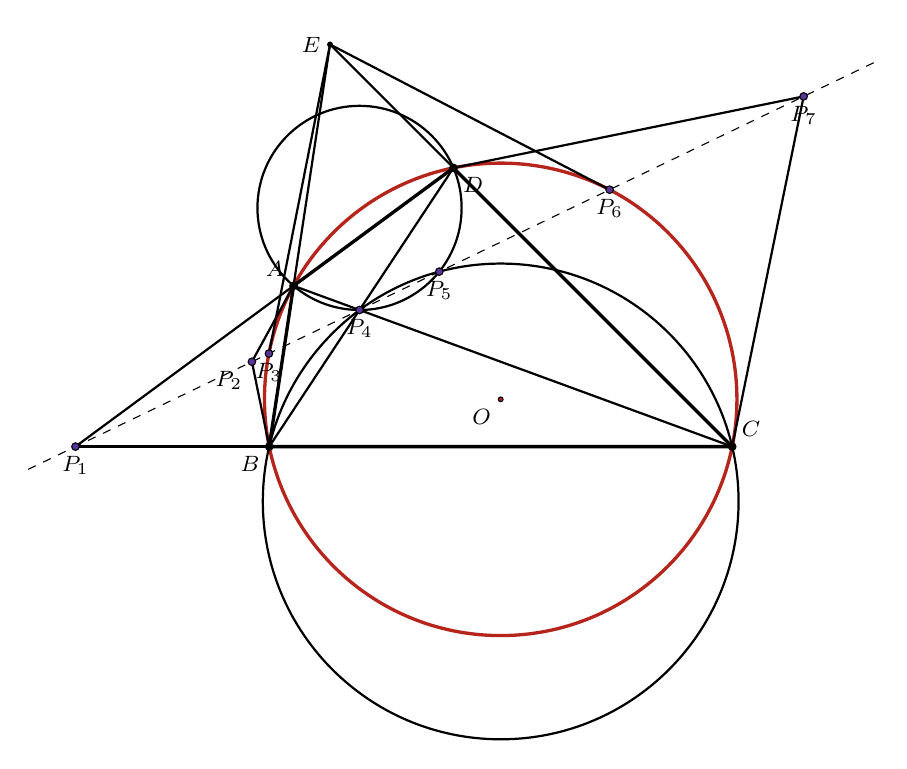
\begin{tikzpicture}[scale=0.6]
    \coordinate (A) at (-4.384520037167606,2.4033277020988573);
    \coordinate (B) at (-4.898979485566357,-1);
    \coordinate (C) at (4.898979485566356,-1);
    \coordinate (D) at (-1,4.898979485566356);
    \coordinate (E) at (-3.6123724356957942,7.51135192126215);
    \coordinate (O) at (0,0);
    \coordinate (p1) at (-9,-1);
    \coordinate (p2) at (-5.265579138398199,0.795964178638951);
    \coordinate (p3) at (-4.90514508446699,0.9693047510093655);
    \coordinate (p4) at (-2.9879263258190374,1.8913369323713356);
    \coordinate (p5) at (-1.2999823794026422,2.703105872097646);
    \coordinate (p6) at (2.305180325661704,4.436906993185929);
    \coordinate (p7) at (6.411934223441692,6.411934223441692);
    \coordinate (v1) at (-10,-1.4809217399960137);
    \coordinate (v2) at (8,7.175669579932235);

    \draw[very thick,BrickRed] (O) circle (5);
    \draw[thick] (-2.9879263258190374,4.052126416957246)
        circle (2.1607894845859104);
    \draw[thick] (0,-2.1607894845859112) circle (5.034623345149588);

    \draw[very thick] (A) -- (B) -- (C) -- (D) -- cycle;
    \draw[thick] (A) -- (C);
    \draw[thick] (B) -- (D);
    \draw[thick] (E) -- (B);
    \draw[thick] (E) -- (C);
    \draw[thick] (p1) -- (C);
    \draw[thick] (p1) -- (D);
    \draw[thick] (p2) -- (A);
    \draw[thick] (p2) -- (B);
    \draw[thick] (p3) -- (E);
    \draw[thick] (p6) -- (E);
    \draw[thick] (p7) -- (C);
    \draw[thick] (p7) -- (D);
    \draw[dashed] (v1) -- (v2);

    \draw[fill=black] (A) circle (0.08)
        node[above left] {\footnotesize $A$};
    \draw[fill=black] (B) circle (0.08)
        node[below left] {\footnotesize $B$};
    \draw[fill=black] (C) circle (0.08)
        node[above right] {\footnotesize $C$};
    \draw[fill=black] (D) circle (0.08)
        node[below right] {\footnotesize $D$};
    \draw[fill=black] (E) circle (0.05)
        node[left] {\footnotesize $E$};
    \draw[fill=BrickRed] (O) circle (0.05)
        node[below left] {\footnotesize $O$};
    \draw[fill=RoyalPurple] (p1) circle (0.08)
        node[below] {\footnotesize $P_1$};
    \draw[fill=RoyalPurple] (p2) circle (0.08)
        node[below left] {\footnotesize $P_2$};
    \draw[fill=RoyalPurple] (p3) circle (0.08)
        node[below] {\footnotesize $P_3$};
    \draw[fill=RoyalPurple] (p4) circle (0.08)
        node[below] {\footnotesize $P_4$};
    \draw[fill=RoyalPurple] (p5) circle (0.08)
        node[below] {\footnotesize $P_5$};
    \draw[fill=RoyalPurple] (p6) circle (0.08)
        node[below] {\footnotesize $P_6$};
    \draw[fill=RoyalPurple] (p7) circle (0.08)
        node[below] {\footnotesize $P_7$};
\end{tikzpicture}
\end{figure}

Here, quadrilateral $ABCD$ is inscribed in the circle with center $O$,
and $E$ and $P_1$ are the points obtained by finding the intersection
between $AB$ and $CD$ and intersection between $AD$ and $BC$
respectively. $P_2$ and $P_7$ are obtained by finding the intersection
between the lines tangent to the circle with center $O$ from $A$ and
$B$ and $C$ and $D$ respectively. Finally, $P_4$ is the intersection
of $AC$ and $BD$ and $P_5$ is the intersection of circumcircles of
$\triangle{P_4AD}$ and $\triangle{P_4BC}$.

I know this sounds a lot at first, but it is actually quite easy to
memorize and notice in problems involving cyclic quadrilaterals.
Now let's prove this thing!

\begin{proof}
Consider the annotated diagram below.

\begin{figure}[H]
\centering
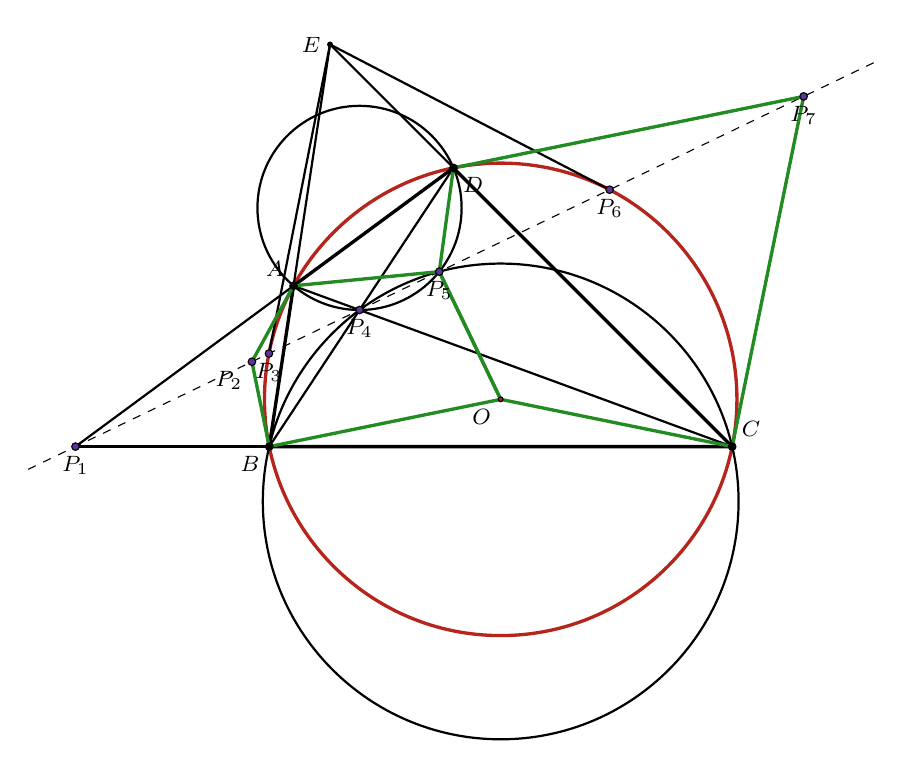
\begin{tikzpicture}[scale=0.6]
    \coordinate (A) at (-4.384520037167606,2.4033277020988573);
    \coordinate (B) at (-4.898979485566357,-1);
    \coordinate (C) at (4.898979485566356,-1);
    \coordinate (D) at (-1,4.898979485566356);
    \coordinate (E) at (-3.6123724356957942,7.51135192126215);
    \coordinate (O) at (0,0);
    \coordinate (p1) at (-9,-1);
    \coordinate (p2) at (-5.265579138398199,0.795964178638951);
    \coordinate (p3) at (-4.90514508446699,0.9693047510093655);
    \coordinate (p4) at (-2.9879263258190374,1.8913369323713356);
    \coordinate (p5) at (-1.2999823794026422,2.703105872097646);
    \coordinate (p6) at (2.305180325661704,4.436906993185929);
    \coordinate (p7) at (6.411934223441692,6.411934223441692);
    \coordinate (v1) at (-10,-1.4809217399960137);
    \coordinate (v2) at (8,7.175669579932235);

    \draw[very thick,BrickRed] (O) circle (5);
    \draw[thick] (-2.9879263258190374,4.052126416957246)
        circle (2.1607894845859104);
    \draw[thick] (0,-2.1607894845859112) circle (5.034623345149588);

    \draw[very thick] (A) -- (B) -- (C) -- (D) -- cycle;
    \draw[thick] (A) -- (C);
    \draw[thick] (B) -- (D);
    \draw[thick] (E) -- (B);
    \draw[thick] (E) -- (C);
    \draw[thick] (p1) -- (C);
    \draw[thick] (p1) -- (D);
    \draw[thick] (p2) -- (A);
    \draw[thick] (p2) -- (B);
    \draw[thick] (p3) -- (E);
    \draw[thick] (p6) -- (E);
    \draw[thick] (p7) -- (C);
    \draw[thick] (p7) -- (D);
    \draw[dashed] (v1) -- (v2);

    \draw[very thick, ForestGreen]
        (A) -- (p2) -- (B) -- (O) -- (p5) -- cycle;
    \draw[very thick, ForestGreen]
        (D) -- (p5) -- (O) -- (C) -- (p7) -- cycle;

    \draw[fill=black] (A) circle (0.08)
        node[above left] {\footnotesize $A$};
    \draw[fill=black] (B) circle (0.08)
        node[below left] {\footnotesize $B$};
    \draw[fill=black] (C) circle (0.08)
        node[above right] {\footnotesize $C$};
    \draw[fill=black] (D) circle (0.08)
        node[below right] {\footnotesize $D$};
    \draw[fill=black] (E) circle (0.05)
        node[left] {\footnotesize $E$};
    \draw[fill=BrickRed] (O) circle (0.05)
        node[below left] {\footnotesize $O$};
    \draw[fill=RoyalPurple] (p1) circle (0.08)
        node[below] {\footnotesize $P_1$};
    \draw[fill=RoyalPurple] (p2) circle (0.08)
        node[below left] {\footnotesize $P_2$};
    \draw[fill=RoyalPurple] (p3) circle (0.08)
        node[below] {\footnotesize $P_3$};
    \draw[fill=RoyalPurple] (p4) circle (0.08)
        node[below] {\footnotesize $P_4$};
    \draw[fill=RoyalPurple] (p5) circle (0.08)
        node[below] {\footnotesize $P_5$};
    \draw[fill=RoyalPurple] (p6) circle (0.08)
        node[below] {\footnotesize $P_6$};
    \draw[fill=RoyalPurple] (p7) circle (0.08)
        node[below] {\footnotesize $P_7$};
\end{tikzpicture}
\end{figure}

First, notice that $P_1$ is the radical center of three circles.
Therefore, $P_1, P_4, P_5$ are collinear. Continuing, notice that
quadrilaterals $AP_2BO$ and $DOCP_7$ are cyclic by construction.
Moreover, the following equations hold.
\begin{align*}
    \angle{AP_3B}
    &= \angle{AP_3P_4} + \angle{P_4P_3B} \\
    &= \angle{ADB} + \angle{ABC}
    = \angle{AOB} \\
    \angle{DP_5C}
    &= 360 - \angle{DP_5P_4} - \angle{P_4P_5C} \\
    &= 180 - \angle{DP_5P_4} + 180 - \angle{P_4P_5C} \\
    &= \angle{DAC} + \angle{DBC}
    = \angle{DOC}
\end{align*}
Therefore, $(A P_2 B O P_5)$ and $(D P_5 O C P_7)$.

Continuing, consider the following equations.
\begin{align*}
    \angle{P_4P_5O}
    &= \angle{P_4P_5B} + \angle{BP_5O}
    &= \angle{ACB} + \angle{BAO}
    = 90^\circ
\end{align*}
Therefore, $P_4P_5 \perp P_5O$ and $E, P_5, O$ are collinear since $E$
is the radical center of $\omega_1, \omega_4, \omega_5$ where
$\omega_4$ and $\omega_5$ are the circle that circumscribe the
pentagons. Because $OP_2$ and $OP_7$ are the diameter of $\omega_4$
and $\omega_5$, $P_1, P_2, P_4, P_5, P_7 \in l$.

Using power of a point theorem, notice that the following equations
hold.
\begin{align*}
    EP_3^2 &= ED \cdot EC = EP_5 \cdot EO \\
    \therefore
    EP_3 : EO &= EP_5 : EP_3 \\
    EP_6^2 &= EA \cdot EB = EP_5 \cdot EO \\
    \therefore
    EP_6 : EO &= EP_5 : EP_6
\end{align*}
Therefore, $\triangle{EP_5P_3} \sim \triangle{EP_3O}$ and
$\triangle{EP_5P_6} \sim \triangle{EP_6O}$. In other words,
$P_3P_5 \perp P_5O$ and $P_6P_5 \perp P_5O$. Thus, the seven points
are collinear.
\end{proof}

This could look a lot, but when you think about it, you can observe
this in most of the problems involving cyclic quadrilaterals.
Many times, three or four of these seven points act as a breakthrough
of the problems. Here is a quick example.

\begin{problem}{2020 KMO Problem 2}{2020 KMO Problem 2}
Given an acute triangle $ABC$, let $H$ and $M$ be the orthocenter
and the midpoint of $BC$ respectively. Let $D$ and $E$ be the
intersection between the circle with diameter $AH$ and sides
$AB$ and $AC$ respectively. Let $P$ be the intersection of
$AH$ and $DE$ and let $Q$ be the intersection of $DM$ and the line
perpendicular to $AH$ that passes through $H$. Show that $P, Q, B$
are collinear.
\end{problem}
\begin{solution}
First, consider the following diagram.

\begin{figure}[H]
\centering
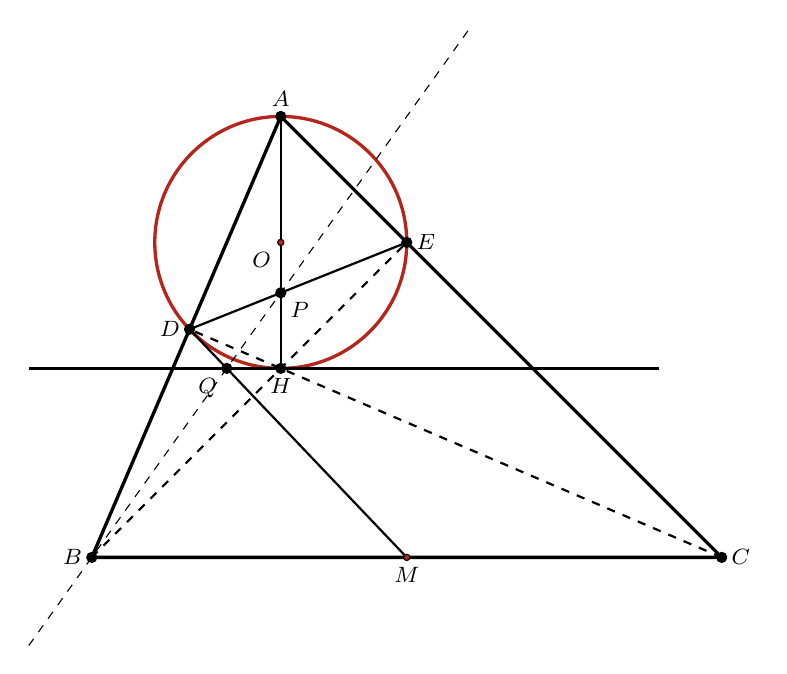
\begin{tikzpicture}[scale=0.8]
    \coordinate (A) at (3,7);
    \coordinate (B) at (0,0);
    \coordinate (C) at (10,0);
    \coordinate (D) at (1.5517241379310345,3.6206896551724137);
    \coordinate (E) at (5,5);
    \coordinate (H) at (3,3);
    \coordinate (M) at (5,0);
    \coordinate (P) at (3,4.2);
    \coordinate (Q) at (2.142857142857143,3);
    \coordinate (R) at (3.378378378378377,4.729729729729727);
    \coordinate (O) at (3,5);
    \coordinate (v1) at (-1,3);
    \coordinate (v2) at (9,3);
    \coordinate (v3) at (-1,-1.4);
    \coordinate (v4) at (6,8.4);

    \draw[very thick,BrickRed] (O) circle (2);

    \draw[very thick] (A) -- (B) -- (C) -- cycle;
    \draw[thick, dashed] (B) -- (E);
    \draw[thick, dashed] (C) -- (D);
    \draw[thick] (D) -- (M);
    \draw[thick] (A) -- (H);
    \draw[thick] (D) -- (E);
    \draw[thick] (v1) -- (v2);
    \draw[dashed] (v3) -- (v4);

    \draw[fill=black] (A) circle (0.08)
        node[above] {\footnotesize $A$};
    \draw[fill=black] (B) circle (0.08)
        node[left] {\footnotesize $B$};
    \draw[fill=black] (C) circle (0.08)
        node[right] {\footnotesize $C$};
    \draw[fill=black] (D) circle (0.08)
        node[left] {\footnotesize $D$};
    \draw[fill=black] (E) circle (0.08)
        node[right] {\footnotesize $E$};
    \draw[fill=black] (H) circle (0.08)
        node[below] {\footnotesize $H$};
    \draw[fill=black] (P) circle (0.08)
        node[below right] {\footnotesize $P$};
    \draw[fill=black] (Q) circle (0.08)
        node[below left] {\footnotesize $Q$};
    \draw[fill=BrickRed] (O) circle (0.05)
        node[below left] {\footnotesize $O$};
    \draw[fill=BrickRed] (M) circle (0.05)
        node[below] {\footnotesize $M$};
\end{tikzpicture}
\end{figure}

Looking at the diagram with respect to cyclic quadrilateral $ADHE$,
the six collinear points can be found. Consider the annotated diagram.

\begin{figure}[H]
\centering
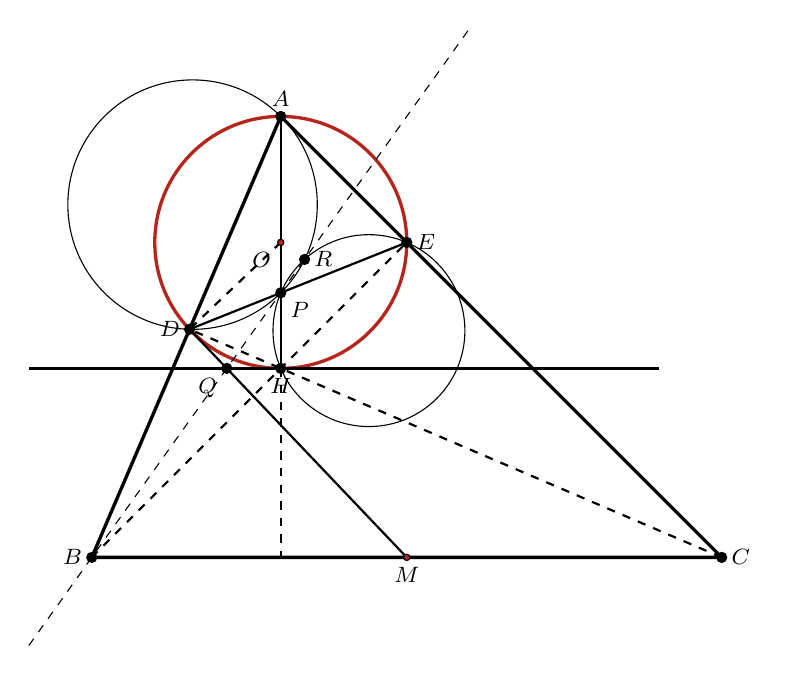
\begin{tikzpicture}[scale=0.8]
    \coordinate (A) at (3,7);
    \coordinate (B) at (0,0);
    \coordinate (C) at (10,0);
    \coordinate (D) at (1.5517241379310345,3.6206896551724137);
    \coordinate (E) at (5,5);
    \coordinate (F) at (3,0);
    \coordinate (H) at (3,3);
    \coordinate (M) at (5,0);
    \coordinate (P) at (3,4.2);
    \coordinate (Q) at (2.142857142857143,3);
    \coordinate (R) at (3.378378378378377,4.729729729729727);
    \coordinate (O) at (3,5);
    \coordinate (v1) at (-1,3);
    \coordinate (v2) at (9,3);
    \coordinate (v3) at (-1,-1.4);
    \coordinate (v4) at (6,8.4);

    \draw[very thick,BrickRed] (O) circle (2);
    \draw (1.6,5.6) circle (1.9798989873223334);
    \draw (4.4,3.6) circle (1.523154621172781);

    \draw[very thick] (A) -- (B) -- (C) -- cycle;
    \draw[thick, dashed] (B) -- (E);
    \draw[thick, dashed] (C) -- (D);
    \draw[thick] (D) -- (M);
    \draw[thick] (A) -- (H);
    \draw[thick] (D) -- (E);
    \draw[thick, dashed] (H) -- (F);
    \draw[thick, dashed] (O) -- (D);
    \draw[thick] (v1) -- (v2);
    \draw[dashed] (v3) -- (v4);

    \draw[fill=black] (A) circle (0.08)
        node[above] {\footnotesize $A$};
    \draw[fill=black] (B) circle (0.08)
        node[left] {\footnotesize $B$};
    \draw[fill=black] (C) circle (0.08)
        node[right] {\footnotesize $C$};
    \draw[fill=black] (D) circle (0.08)
        node[left] {\footnotesize $D$};
    \draw[fill=black] (E) circle (0.08)
        node[right] {\footnotesize $E$};
    \draw[fill=black] (H) circle (0.08)
        node[below] {\footnotesize $H$};
    \draw[fill=black] (P) circle (0.08)
        node[below right] {\footnotesize $P$};
    \draw[fill=black] (Q) circle (0.08)
        node[below left] {\footnotesize $Q$};
    \draw[fill=black] (R) circle (0.08)
        node[right] {\footnotesize $R$};
    \draw[fill=BrickRed] (O) circle (0.05)
        node[below left] {\footnotesize $O$};
    \draw[fill=BrickRed] (M) circle (0.05)
        node[below] {\footnotesize $M$};
\end{tikzpicture}
\end{figure}

From here, notice that with $\angle{ADH} = \alpha$, we have
$\alpha = \angle{DEH} = \angle{DHQ} = \angle{DCB}$. Moreover,
$\angle{DMB} = 2\alpha = \angle{DOH}$. In other words,
$OD \perp DM$ and $B, P, Q$ are three of the seven points.

Continuing, consider the new point $R$. Notice that because
$\angle{DRP} + \angle{PRH} = \angle{DAH} + \angle{DEH} = \angle{DOH}$,
$(DORHQ)$. Moreover, notice that $\angle{ORP} = \angle{ORD} +
\angle{DRP} = \angle{OHD} + \angle{DAH} = 90^\circ$.
Because $\angle{QRO} = 90^\circ$, $Q, P, R$ are collinear and
$B, Q, P, R$ are also collinear by radical axis. Therefore,
$P, Q, B$ are collinear.
\end{solution}

This problem is now easy with six collinear points! There are many
different ways to solve this problem such as using homothety
and pole and polar, but I think this method is the most
straightforward. This is it for this section! In the next section,
we will discuss another very important topic isogonal conjugate.

\end{document}


